\clearpage

\section{Presentazione Liste, Tuple, Dizionari, Set}

Questo capitolo esplorerà le quattro principali strutture dati incorporate nel linguaggio: \textbf{liste, tuple, dizionari, set}. Queste strutture rappresentano modi diversi di organizzare le informazioni, ognuna di esse con caratteristiche uniche e caso d'uso specifico.\\



Il modo di presentarle sarà uguale alle sezioni precedenti, quindi introduzione teorica sugli aspetti peculiari con relativi esempi, rappresentazione pratica dell'utilizzo con relativi approfondimenti sui metodi, esercizi per consolidamento della parte teorica, correlati con relative soluzioni.\\


\percorsoApprendimento{Strutture dati in Python}{
Questa è una introduzione alle strutture dati fondamentali. Nei capitoli successivi approfondiremo ciascuna struttura, esplorando algoritmi avanzati e pattern di programmazione che le utilizzano in contesti reali.
}



\subsection{Liste}\label{ListeCap1}
\subsubsection{Definizione e Caratteristiche Principali}

Le liste sono una delle strutture dati più versatili e utilizzate in Python. Una lista è una sequenza ordinata di "\textbf{\nameref{mutableImmutable}}" di elementi che può contenere valori di qualsiasi tipo.

\begin{tcolorbox}[colback=blue!5!white,colframe=blue!75!black,title=Caratteristiche principali delle liste]
\begin{itemize}
    \item \textbf{Delimitate da parentesi quadre}: Le liste si creano racchiudendo gli elementi tra parentesi quadre [ ]
    \item \textbf{Ordinate}: Gli elementi mantengono l'ordine in cui sono stati inseriti
    \item \textbf{Mutabili}: È possibile modificare, aggiungere o rimuovere elementi dopo la creazione
    \item \textbf{Indicizzate}: Si può accedere agli elementi tramite indici numerici, partendo da 0
    \item \textbf{Eterogenee}: Possono contenere elementi di tipi diversi (numeri, stringhe, booleani, altre liste, ecc.)
    \item \textbf{Duplicati ammessi}: Possono contenere elementi ripetuti
\end{itemize}
\end{tcolorbox}

Le liste sono estremamente utili per gestire collezioni di dati correlati, come una serie di numeri, un elenco di nomi, oppure qualsiasi altro raggruppamento di valori che devono mantenere un ordine specifico.

\begin{esempio}
Una lista può rappresentare:
\begin{itemize}
    \item Una lista della spesa: \texttt{["pane", "latte", "uova", "mele"]}
    \item Una sequenza di numeri: \texttt{[1, 2, 3, 4, 5]}
    \item Un insieme di valori di tipo diverso: \texttt{["Mario", 25, 1.75, True]}
    \item I giorni della settimana: \texttt{["Lunedì", "Martedì", "Mercoledì", "Giovedì", "Venerdì", "Sabato", "Domenica"]}
\end{itemize}
\end{esempio}

\begin{nota}
In molti altri linguaggi di programmazione, strutture simili alle liste di Python sono chiamate "array". Tuttavia, le liste Python sono più flessibili degli array tradizionali, poiché possono contenere elementi di tipi diversi e si ridimensionano automaticamente.
\end{nota}

\begin{center}
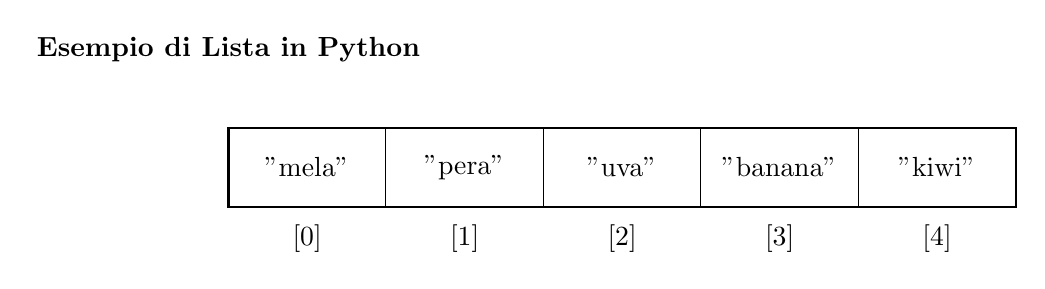
\begin{tikzpicture}
    % Titolo
    \node[font=\bfseries] at (0,2) {Esempio di Lista in Python};
    
    % Disegna i box della lista
    \draw[thick] (0,0) rectangle (10,1);
    \draw (2,0) -- (2,1);
    \draw (4,0) -- (4,1);
    \draw (6,0) -- (6,1);
    \draw (8,0) -- (8,1);
    
    % Contenuto della lista
    \node at (1,0.5) {"mela"};
    \node at (3,0.5) {"pera"};
    \node at (5,0.5) {"uva"};
    \node at (7,0.5) {"banana"};
    \node at (9,0.5) {"kiwi"};
    
    % Indici
    \node[below] at (1,-0.1) {[0]};
    \node[below] at (3,-0.1) {[1]};
    \node[below] at (5,-0.1) {[2]};
    \node[below] at (7,-0.1) {[3]};
    \node[below] at (9,-0.1) {[4]};
\end{tikzpicture}
\end{center}


Python offre anche un secondo sistema di indicizzazione, utilizzando numeri negativi, che permette di accedere agli elementi partendo dalla fine della lista:\\

Gli indici negativi sono molto utili quando si vuole accedere agli elementi partendo dalla fine della lista, senza dover conoscere la lunghezza totale della lista. Ad esempio, \texttt{[-1]} si riferisce sempre all'ultimo elemento, indipendentemente da quanti elementi contiene la lista.
Con l'unica differenza che contando al contrario non bisognerà arrivare a \texttt{[0]}. ma soltanto a \texttt{[-1]}.


\begin{center}
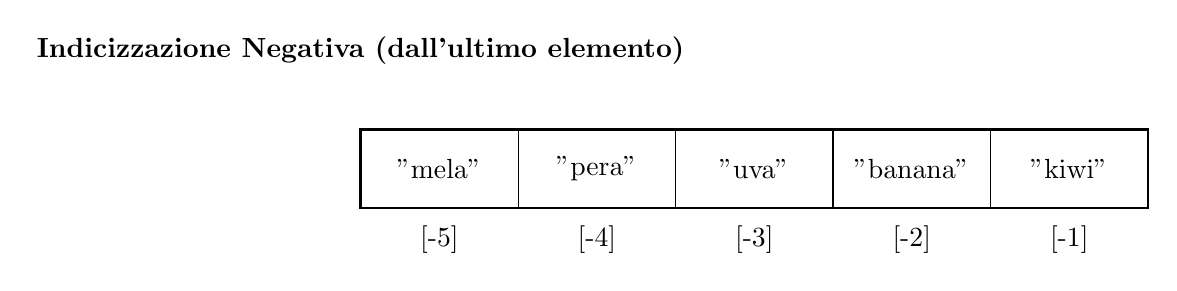
\begin{tikzpicture}
% Titolo
\node[font=\bfseries] at (0,2) {Indicizzazione Negativa (dall'ultimo elemento)};
% Disegna i box della lista
\draw[thick] (0,0) rectangle (10,1);
\draw (2,0) -- (2,1);
\draw (4,0) -- (4,1);
\draw (6,0) -- (6,1);
\draw (8,0) -- (8,1);

% Contenuto della lista
\node at (1,0.5) {"mela"};
\node at (3,0.5) {"pera"};
\node at (5,0.5) {"uva"};
\node at (7,0.5) {"banana"};
\node at (9,0.5) {"kiwi"};

% Indici negativi
\node[below] at (1,-0.1) {[-5]};
\node[below] at (3,-0.1) {[-4]};
\node[below] at (5,-0.1) {[-3]};
\node[below] at (7,-0.1) {[-2]};
\node[below] at (9,-0.1) {[-1]};
\end{tikzpicture}
\end{center}


Per comprendere meglio come funziona l'indicizzazione delle liste in Python, osserviamo una rappresentazione in stile Python Tutor che mostra visivamente la corrispondenza tra indici ed elementi:


\begin{center}
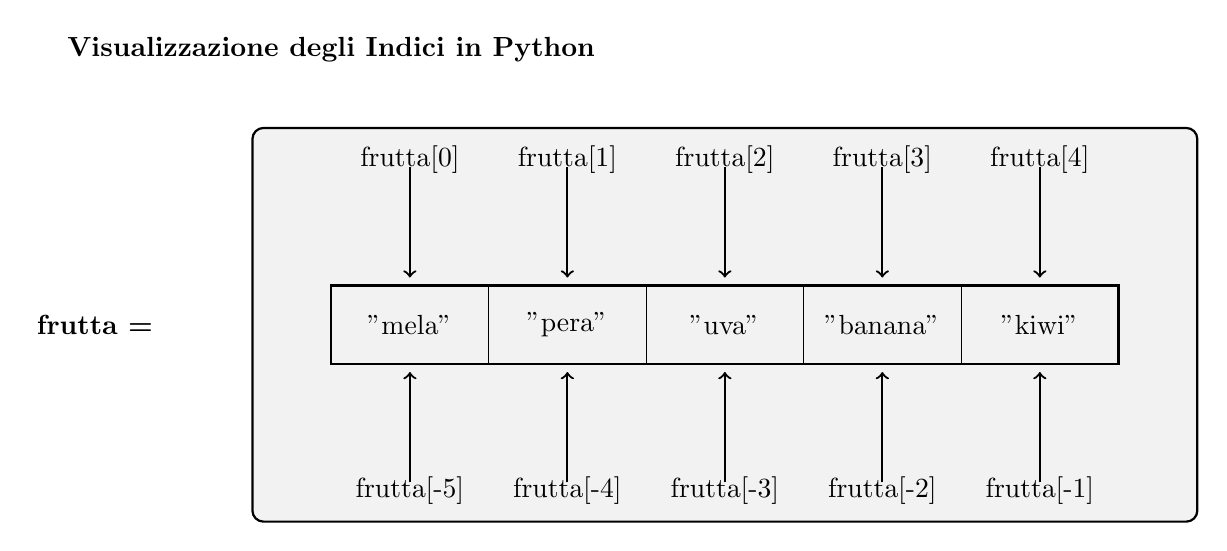
\begin{tikzpicture}
    % Titolo
    \node[font=\bfseries] at (0,4) {Visualizzazione degli Indici in Python};
    
    % Creare una scatola che conterrà la lista e gli indici
    \draw[rounded corners, thick, fill=gray!10] (-1,-2) rectangle (11,3);
    
    % Nome della variabile
    \node[font=\bfseries, align=right] at (-3, 0.5) {frutta =};
    
    % Disegna i box della lista
    \draw[thick] (0,0) rectangle (10,1);
    \draw (2,0) -- (2,1);
    \draw (4,0) -- (4,1);
    \draw (6,0) -- (6,1);
    \draw (8,0) -- (8,1);
    
    % Contenuto della lista
    \node at (1,0.5) {"mela"};
    \node at (3,0.5) {"pera"};
    \node at (5,0.5) {"uva"};
    \node at (7,0.5) {"banana"};
    \node at (9,0.5) {"kiwi"};
    
    % Indici positivi (sopra) 
    \foreach \x/\pos in {0/0, 1/2, 2/4, 3/6, 4/8} {
        \draw[thick, ->] (\pos+1,2.5) -- (\pos+1,1.1);
        \node[above] at (\pos+1,2.3) {frutta[\x]};
    }
    
    % Indici negativi (sotto) -
    \foreach \x/\pos in {-5/0, -4/2, -3/4, -2/6, -1/8} {
        \draw[thick, ->] (\pos+1,-1.5) -- (\pos+1,-0.1);
        \node[below] at (\pos+1,-1.3) {frutta[\x]};
    }
\end{tikzpicture}
\end{center}


Questa visualizzazione mostra:
\begin{itemize}
\item Come ogni elemento della lista può essere accessibile utilizzando sia un indice positivo sia un indice negativo
\item \texttt{frutta[0]} e \texttt{frutta[-5]} si riferiscono entrambi al primo elemento ("mela")
\item \texttt{frutta[4]} e \texttt{frutta[-1]} si riferiscono entrambi all'ultimo elemento ("kiwi")
\end{itemize}



Utilizzando la lista \texttt{frutta = ["mela", "pera", "uva", "banana", "kiwi"]}:

\begin{lstlisting}[language=Python]
frutta[0]   # restituisce "mela" (primo elemento)
frutta[2]   # restituisce "uva" (terzo elemento)
frutta[-1]  # restituisce "kiwi" (ultimo elemento)
frutta[-2]  # restituisce "banana" (penultimo elemento)
\end{lstlisting}



\vspace{0.3cm}
A differenza di altre strutture dati che vedremo più avanti (come le tuple), le liste sono \textit{mutabili}, il che significa che è possibile modificare il loro contenuto dopo la creazione. Questa caratteristica le rende ideali per situazioni in cui i dati devono cambiare nel tempo.
\begin{attenzione}
Gli indici delle liste in Python iniziano da 0, non da 1. Quindi, il primo elemento di una lista si trova all'indice 0, il secondo all'indice 1, e così via. Questo è un concetto fondamentale che si ritrova in molti linguaggi di programmazione.
\end{attenzione}

\subsection{L'Indicizzazione delle Liste in Python}\label{IndicizzazioneListe}

\subsubsection{Un modello matematico per comprendere gli indici}

In Python, l'indicizzazione delle liste rappresenta uno dei concetti fondamentali che permette di accedere agli elementi di una collezione ordinata. Ciò che rende particolarmente elegante questo sistema è la possibilità di indicizzare in due direzioni: dalla sinistra verso destra (con indici positivi) e dalla destra verso sinistra (con indici negativi).

\paragraph{Il Modello dell'Anello Chiuso}
Possiamo immaginare una lista Python come un anello chiuso di elementi, simile a una struttura circolare. In matematica, quando abbiamo un insieme finito di elementi ordinati che può essere percorso ciclicamente, possiamo rappresentarlo come un insieme chiuso modulo il numero di elementi.

Per una lista di lunghezza $n$, abbiamo la seguente relazione fondamentale:

\begin{center}
\fbox{L'elemento all'indice $i$ è identico all'elemento all'indice $(i - n)$}
\end{center}

In altre parole, se abbiamo una lista di 5 elementi, l'elemento all'indice 0 è lo stesso dell'elemento all'indice $-5$, l'elemento all'indice 1 è lo stesso dell'elemento all'indice $-4$, e così via.

\paragraph{Rappresentazione Visiva}
Consideriamo una lista \texttt{frutti = ["mela", "banana", "arancia", "kiwi", "uva"]}:

\begin{center}
\begin{tabular}{|c|c|c|c|c|c|}
\hline
\textbf{Indici positivi:} & 0 & 1 & 2 & 3 & 4 \\
\hline
\textbf{Elementi:} & "mela" & "banana" & "arancia" & "kiwi" & "uva" \\
\hline
\textbf{Indici negativi:} & -5 & -4 & -3 & -2 & -1 \\
\hline
\end{tabular}
\end{center}

Osserviamo che:
\begin{itemize}
    \item L'indice 0 corrisponde a -5 \quad ($0 - 5 = -5$)
    \item L'indice 1 corrisponde a -4 \quad ($1 - 5 = -4$)
    \item L'indice 2 corrisponde a -3 \quad ($2 - 5 = -3$)
    \item L'indice 3 corrisponde a -2 \quad ($3 - 5 = -2$)
    \item L'indice 4 corrisponde a -1 \quad ($4 - 5 = -1$)
\end{itemize}

\paragraph{La Formula Matematica}
Per qualsiasi lista di lunghezza $n$, la relazione tra indici positivi e negativi segue questa formula:

\begin{align}
\text{indice\_negativo} &= \text{indice\_positivo} - n\\
\text{indice\_positivo} &= \text{indice\_negativo} + n
\end{align}

Questa relazione algebrica è esattamente come operare in aritmetica modulare, dove i numeri ``avvolgono'' dopo aver raggiunto una certa dimensione.

\subsubsection{Vantaggi dell'indicizzazione bidirezionale}

L'indicizzazione negativa risolve un problema comune: accedere agli ultimi elementi di una lista senza conoscerne la lunghezza esatta.

Pensa a quante volte in programmazione abbiamo bisogno dell'ultimo elemento o degli ultimi elementi. Utilizzando indici negativi:

\begin{itemize}
    \item \texttt{lista[-1]} $\rightarrow$ sempre l'ultimo elemento
    \item \texttt{lista[-2]} $\rightarrow$ sempre il penultimo elemento
    \item \texttt{lista[-3]} $\rightarrow$ sempre il terzultimo elemento
\end{itemize}

Senza questa funzionalità, dovremmo scrivere \texttt{lista[len(lista)-1]} per ottenere l'ultimo elemento, una sintassi molto più verbosa.

\subsubsection{Esempi pratici}

\begin{lstlisting}[style=pythonstyle]
numeri = [10, 20, 30, 40, 50]

# Accesso con indici positivi
print(numeri[0])  # 10 (primo elemento)
print(numeri[2])  # 30 (terzo elemento)

# Accesso con indici negativi
print(numeri[-1])  # 50 (ultimo elemento)
print(numeri[-3])  # 30 (terzultimo elemento)

# Relazione matematica
for i in range(len(numeri)):
    print(f"numeri[{i}] = numeri[{i-len(numeri)}] = {numeri[i]}")
\end{lstlisting}

Questo codice dimostra che \texttt{numeri[i]} è sempre uguale a \texttt{numeri[i-len(numeri)]}.

\subsubsection{Il concetto di insieme ciclico chiuso}

Matematicamente, possiamo vedere l'indicizzazione delle liste come un'operazione su un insieme ciclico chiuso $\mathbb{Z}/n\mathbb{Z}$ (i numeri interi modulo $n$). Ogni elemento ha esattamente due identificatori: uno positivo e uno negativo.

Questo concetto di ciclicità è particolarmente potente perché ci permette di:
\begin{enumerate}
    \item \textbf{Navigare bidirezionalmente}: possiamo pensare alla lista sia in avanti che all'indietro
    \item \textbf{Esprimere relazioni posizionali}: possiamo esprimere la posizione di un elemento rispetto all'inizio (indici positivi) o rispetto alla fine (indici negativi)
    \item \textbf{Sfruttare la modularità}: l'indicizzazione si comporta come un orologio circolare, dove dopo il 12 torniamo all'1
\end{enumerate}

\begin{nota}
È importante notare che, nonostante questa apparente ``ciclicità'' nell'indicizzazione, Python non permette di usare indici arbitrariamente grandi per ``avvolgere'' la lista. Se proviamo ad accedere a \texttt{lista[len(lista)]} o \texttt{lista[-len(lista)-1]}, otterremo un errore \texttt{IndexError}.

La ciclicità esiste solo nel modello concettuale, non nell'implementazione pratica dell'accesso agli elementi.
\end{nota}

\subsubsection{Conclusione}

L'indicizzazione delle liste in Python può essere vista come un'applicazione dell'aritmetica modulare, dove l'elemento alla posizione $i$ coincide con l'elemento alla posizione $i-n$. Questa doppia indicizzazione offre una flessibilità notevole, permettendo di riferirsi agli elementi sia dalla prospettiva dell'inizio della lista che dalla sua fine.

Questa caratteristica, apparentemente semplice, è un esempio della filosofia di Python: rendere le operazioni comuni immediate ed eleganti, riducendo la verbosità e aumentando la leggibilità del codice.



%Da rivedere questa parte per chiarimenti